\documentclass[12pt]{beamer}
%
% Choose how your presentation looks.
%
% For more themes, color themes and font themes, see:
% http://deic.uab.es/~iblanes/beamer_gallery/index_by_theme.html
%

\mode<presentation>
{
  \usetheme{Madrid}      % or try Darmstadt, Madrid, Warsaw, ...
  \usecolortheme{beaver} % or try albatross, beaver, crane, ...
  \usefonttheme{default}  % or try serif, structurebold, ...
  \setbeamertemplate{navigation symbols}{}
  \setbeamertemplate{caption}[numbered]
} 
\usepackage{pifont}
\usepackage[bookmarks]{hyperref}
\usepackage[backend=bibtex]{biblatex}
\usepackage{braket}
\usepackage{qrcode}
\usepackage{empheq}
\usepackage{amsmath,amsfonts,amsthm,bm}
\addbibresource{bibliography.bib}
\newtheorem*{remark}{Remark}
\usepackage[italian]{babel}
\usepackage[utf8x]{inputenc}

\title[Deepfake & IA]{Deepfake: quando la finzione diventa credibile}
\author{Marzio De Corato}
\date{\today}



\begin{document}

\usebackgroundtemplate{%
  \includegraphics[width=\paperwidth,height=\paperheight]{Pic/Cover_image.png}%
}
\begin{frame}
  \vspace{6.5cm}\titlepage
\end{frame}
% qui azzeri lo sfondo
\usebackgroundtemplate{}
% =========================================================
% OUTLINE
% =========================================================
\begin{frame}{Outline}
  \small
    \tableofcontents
\end{frame}

% =========================================================
\section{Introduzione e definizioni}
% =========================================================
\begin{frame}{Contesto}
  \begin{alertblock}{Motivazione}
    \begin{itemize}
      \item Negli ultimi 8 anni i modelli di generazione sono passati da semplici face‐swap a pipeline multimodali (testo, immagine, audio, video) in tempo reale anche su smartphone.
      \item Clonare una voce convincente costa meno di 10 € in risorse cloud, rendendo l’IA accessibile a chiunque.
      \item Oggi i deepfake non sono più un “giocattolo”: servono nel marketing, nei videogame, nel cinema e, purtroppo, nella disinformazione.
    \end{itemize}
  \end{alertblock}
\end{frame}

\begin{frame}{Definizioni}
\small
  \begin{alertblock}{Deepfake}
    Contenuto multimediale (video, audio, immagine) creato o alterato da modelli di Intelligenza Artificiale Generativa, con l’obiettivo di farlo sembrare reale. Il termine nasce su Reddit nel 2017 e oggi include qualunque manipolazione neurale sofisticata \cite{nsa_definition}.
  \end{alertblock}
  \begin{alertblock}{Intelligenza Artificiale}
    Disciplina che sviluppa sistemi capaci di funzioni cognitive umane (ragionamento, apprendimento, pianificazione) tramite algoritmi e grandi volumi di dati \cite{nist_definition_ai}.
  \end{alertblock}
  \begin{alertblock}{IA Generativa}
    Sottoinsieme dell’IA specializzato nella creazione di nuovi dati (immagini, testo, audio, video), a differenza dell’IA predittiva che “riempie spazi vuoti”.
  \end{alertblock}
\end{frame}

\begin{frame}{Definizioni}
  \begin{alertblock}{Foundation Model}
    Modelli di grandi dimensioni (miliardi di parametri) addestrati su dataset generici e riadattabili a diversi compiti tramite prompt engineering (es. GPT-4o, LLaVA-3).
  \end{alertblock}
  \begin{alertblock}{Normativa: Realistico vs Stilizzato}
    Secondo l’AI Act UE (\S52), se il contenuto “appare reale” serve un’etichetta obbligatoria; se è manifestamente “stilizzato” (cartoon, illustrazioni), bastano avvertenze generiche.
  \end{alertblock}
\end{frame}

% =========================================================
\section{Storia del fenomeno}
% =========================================================
\begin{frame}
\Huge
\begin{center}
Storia del fenomeno
\end{center}
\end{frame}



\begin{frame}{Never trust quotes on the internet -Abraham Lincoln}
  \begin{center}
    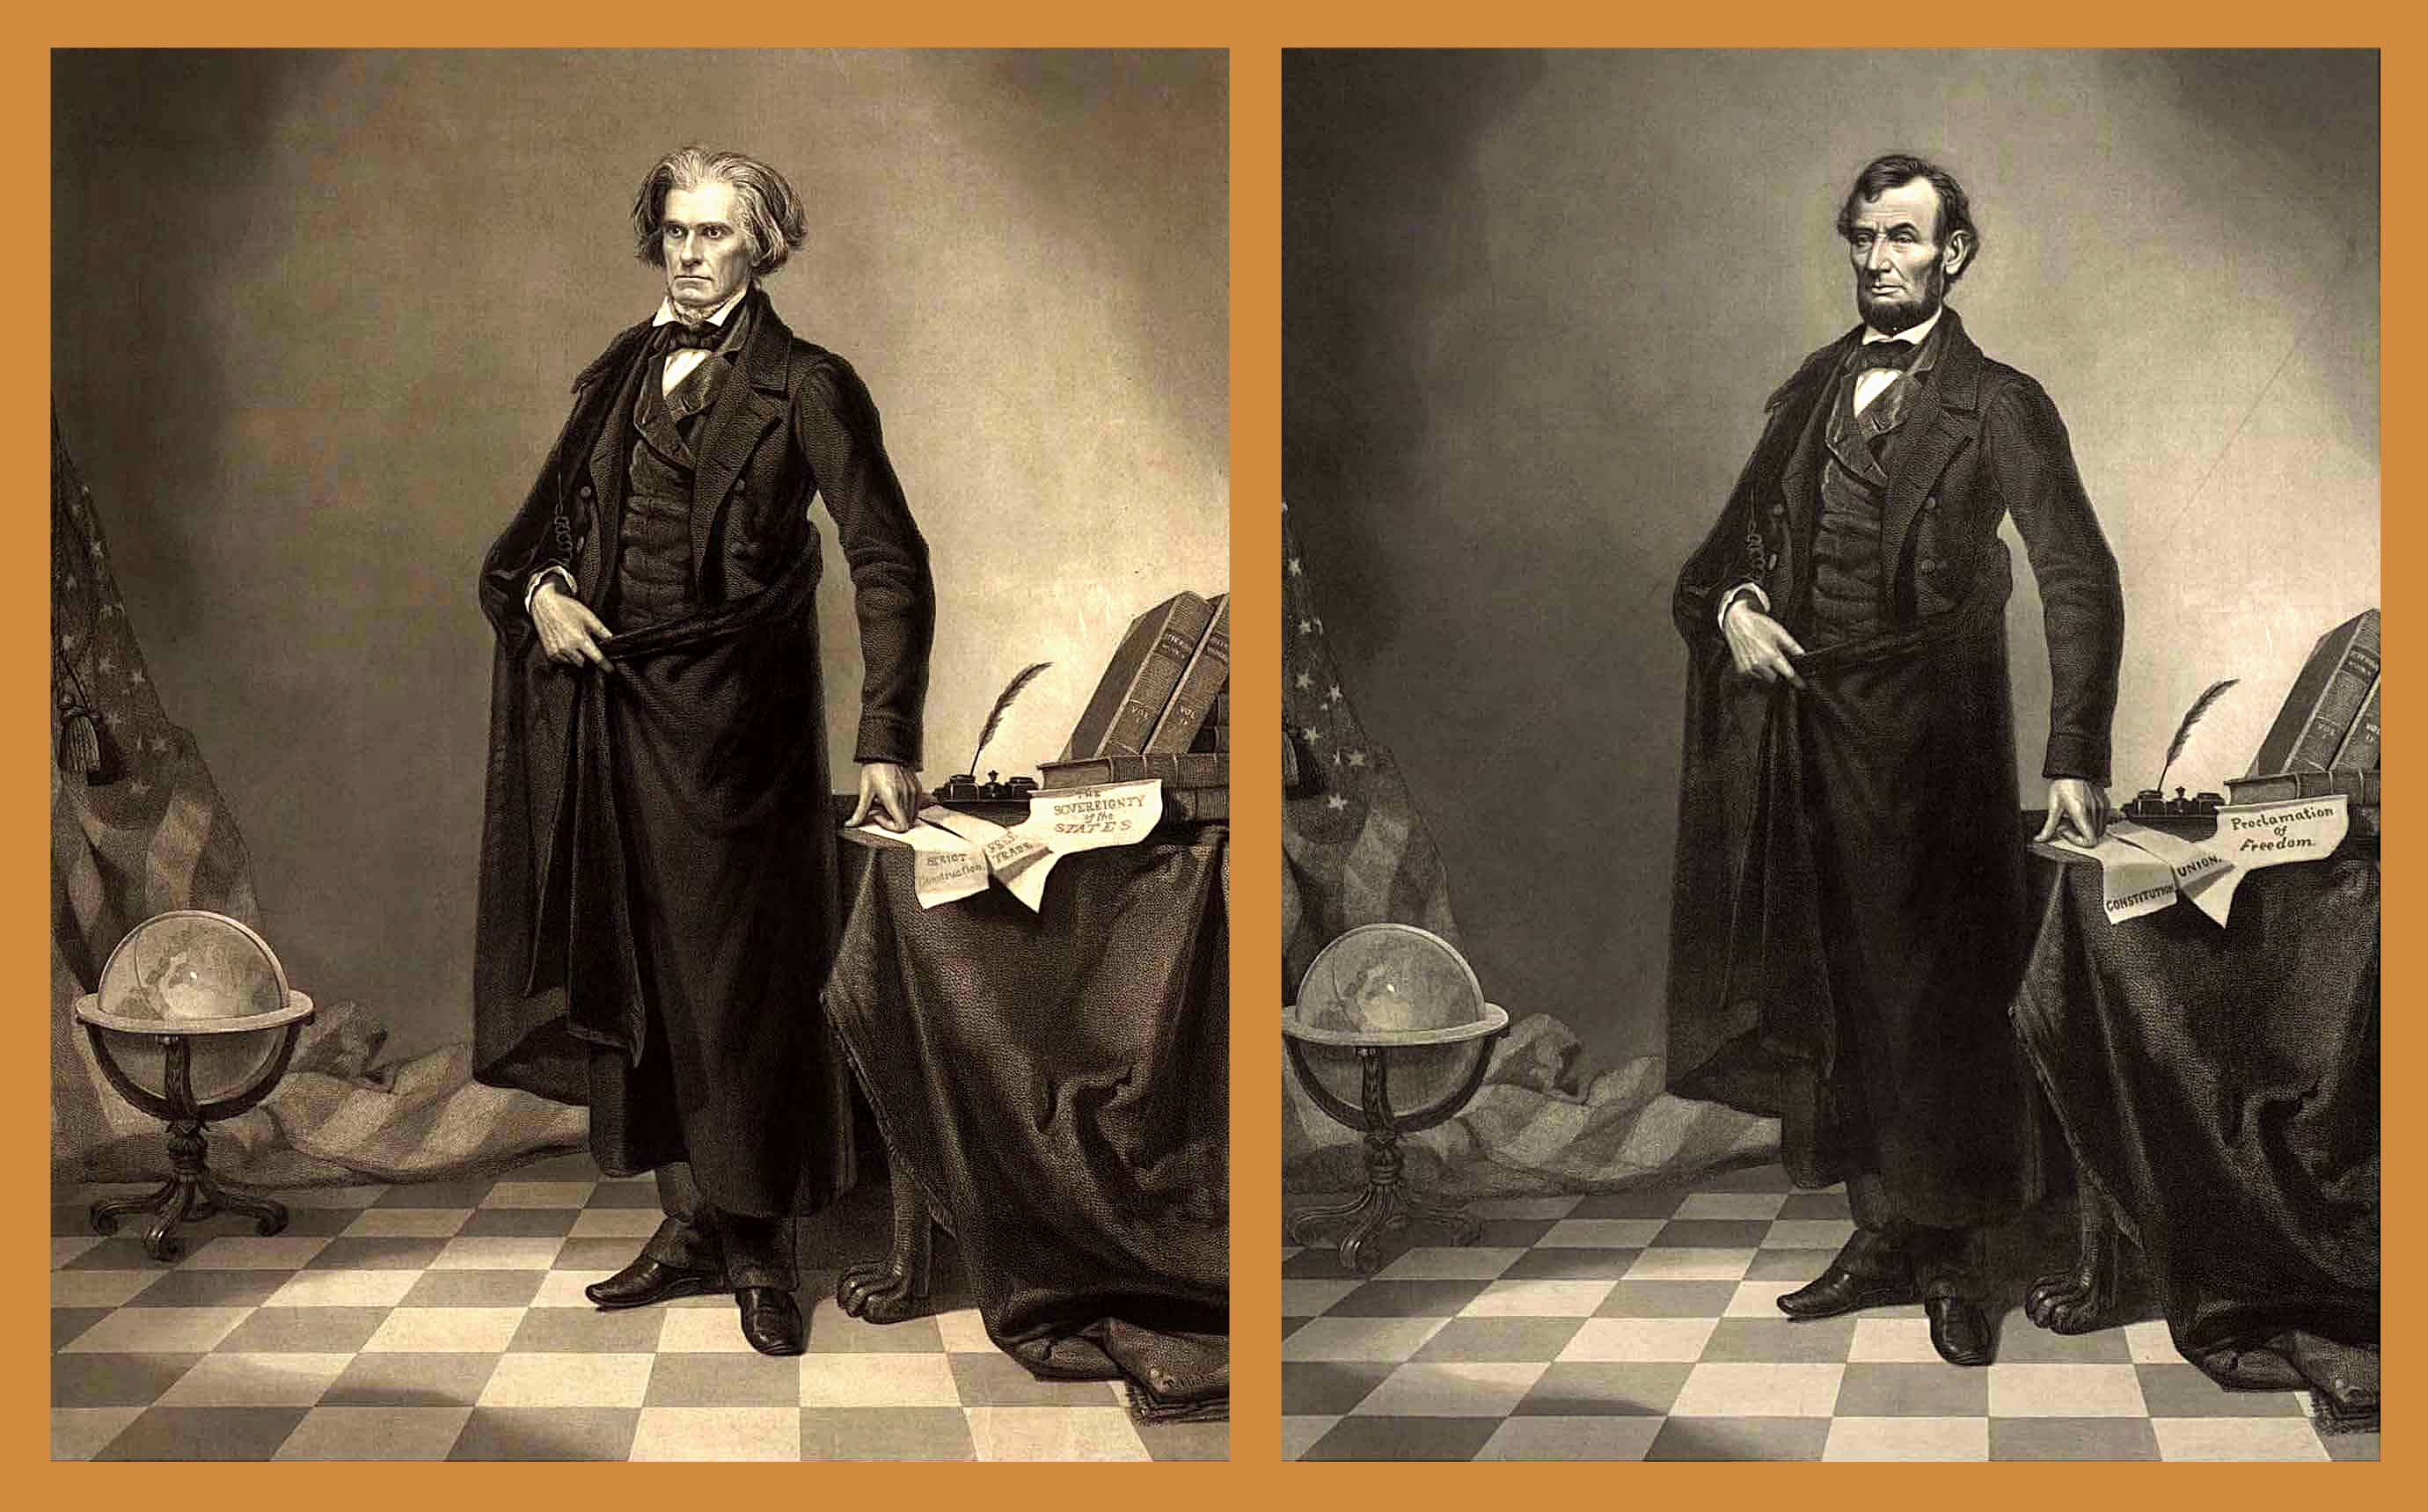
\includegraphics[width=0.85\textwidth]{Pic/Licon_deepfake.jpg}
  \end{center}
\end{frame}



\begin{frame}{Timeline 1860–2025 (1/3)}
  \begin{alertblock}{Origini pre-IA}
    \begin{itemize}
      \item \textbf{1860 – Lincoln/Calhoun:} primi esperimenti di manipolazione fotografica mediante fusione di negativi su lastra, utilizzati come strumento di propaganda politica.
      \item \textbf{1917 – Fate di Cottingley:} due ragazze manipolano immagini con creature fantastiche; il caso diventa virale e crea la prima grande bufala fotografica.
      \item \textbf{1997 – Video Rewrite:} tecniche di warping labiale basate su Hidden Markov Models, antenato delle moderne manipolazioni video neurali.\cite{video_rewrite}
    \end{itemize}
  \end{alertblock}
\end{frame}




\begin{frame}{Timeline 1860–2025 (2/3)}
  \begin{alertblock}{Era delle GAN e social}
    \begin{itemize}
      \item \textbf{2014:} Goodfellow et al. introducono le GAN, consentendo la generazione di immagini realistiche tramite competizione fra due reti neurali.
      \item \textbf{2016:} scandalo Cambridge Analytica dimostra il potere del \emph{profiling} psicografico unito a messaggi persuasivi dinamici.\cite{cambridge_vox}
      \item \textbf{2017:} nasce il subreddit \texttt{/r/deepfakes}; i primi face‐swap pornografici si diffondono rapidamente.
      \item \textbf{2017:} Università di Washington pubblica un deepfake di Obama, primo video virale generato da IA.\cite{reuters_fake}
    \end{itemize}
  \end{alertblock}
\end{frame}

\begin{frame}{Timeline 1860–2025 (3/3)}
  \begin{alertblock}{Diffusione di massa e casi recenti}
    \begin{itemize}
      \item \textbf{2020:} “Cheapfake” su Nancy Pelosi, manipolazione di velocità audio/video per creare falsi compromettenti.
      \item \textbf{2023:} Stable Diffusion 2\&3 democratizzano immagini HD su GPU consumer; Google introduce SynthID, watermark latente resistente.\cite{fcc_robocall}
      \item \textbf{2024:} robocall deepfake di Joe Biden nelle primarie del New Hampshire, uso di voice cloning per truffe politiche.\cite{fcc_robocall}
      \item \textbf{2025:} LVD-XT genera video a 360° in 4 passi; prototipi di watermark hardware-level su ARM.
      \item \textbf{2025:} truffa CFO a Hong Kong con sei volti deepfake su Teams → 35 M USD; operazione “Spamouflage” a Taiwan smantellata da Meta.\cite{cse_canada_2025}\cite{meta_report}
    \end{itemize}
  \end{alertblock}
\end{frame}

% =========================================================
\section{Case studies}
% =========================================================

\begin{frame}
\Huge
\begin{center}
Case studies
\end{center}
\end{frame}

\begin{frame}{Case study: Cambridge Analytica }
  \begin{alertblock}{Raccolta massiva di dati}
    \begin{itemize}
      \item 2014: lancio dell’app “thisisyourdigitallife” sviluppata da Aleksandr Kogan.
      \item Oltre 270 000 utenti installarono volontariamente l’app, ma furono raccolti anche i dati dei loro amici (~87 M profili) senza consenso diretto.
      \item Tipologie di dati acquisiti: like, preferenze, informazioni demografiche, network sociali e interazioni online.
    \end{itemize}
  \end{alertblock}
  \begin{alertblock}{Compliance apparente}
    \begin{itemize}
      \item I dati venivano presentati come “uso accademico” da parte di ricercatori dell’Università di Cambridge (estrenea alla vicenda)
      \item Facebook permise inizialmente l’accesso via API fino al 2015, prima di restringere drasticamente i permessi.
    \end{itemize}
  \end{alertblock}
\end{frame}

\begin{frame}{Case study: Cambridge Analytica}
  \begin{alertblock}{Profilazione psicografica \& Microtargeting}
    \begin{itemize}
      \item Applicazione del modello OCEAN per profilare personalità individuali.
      \item Segmentazione dell’elettorato in gruppi target con messaggi ultra‐personalizzati (Brexit, Trump).
      \item A/B test su decine di varianti di annunci per massimizzare engagement.\cite{cambridge_vox}
    \end{itemize}
  \end{alertblock}
  \begin{alertblock}{Ruolo dell’Università di Cambridge}
    \begin{itemize}
      \item Kogan lavorava presso Cambridge, ma l’app fu sviluppata e distribuita senza alcuna approvazione o supervisione ufficiale.
      \item Cambridge ha preso le distanze, avviato indagini interne e dichiarato di non aver mai tratto vantaggio dai dati.
    \end{itemize}
  \end{alertblock}
\end{frame}




\begin{frame}{Case study: “Mia Ash” }
  \begin{alertblock}{Chi era “Mia Ash”?}
    \begin{itemize}
      \item Synthetic persona creata nel 2016 dall’APT33 (OilRig).
      \item Foto e informazioni rubate da profili reali per dare credibilità.
      \item Profili LinkedIn e Facebook plausibili, con background professionale fittizio.
      \item Video preregistrati e audio deepfake per simulare colloqui di lavoro.\cite{mia_secureworks}
    \end{itemize}
  \end{alertblock}
  \begin{alertblock}{Obiettivi dell’attacco}
    \begin{itemize}
      \item Infiltrarsi in aziende del settore oil & gas.
      \item Ottenere informazioni strategiche e credenziali di accesso.
      \item Stabilire un canale di comunicazione fidato per il payload.
    \end{itemize}
  \end{alertblock}
\end{frame}

\begin{frame}{Case study: “Mia Ash”}
  \begin{alertblock}{Modus operandi}
    \begin{itemize}
      \item Primo contatto: inviti su LinkedIn e messaggi diretti via Facebook.
      \item Chat video fake per guadagnare fiducia (deepfake audio/video).
      \item Invio di un documento Word malevolo che installa PupyRAT.
      \item Accesso persistente ai sistemi aziendali e movimento laterale.
      \item Evasione: utilizzo di tool di sistema per ridurre tracce (“living off the land”).
    \end{itemize}
  \end{alertblock}
  \begin{alertblock}{Implicazioni 2025}
    \begin{itemize}
      \item Oggi creare synthetic personas richiede pochi click con tool IA multimodali.
    \end{itemize}
  \end{alertblock}
\end{frame}


% =========================================================
\section{IA Predittiva vs IA Generativa}
% =========================================================

\begin{frame}
\Huge
\begin{center}
IA Predittiva vs IA Generativa
\end{center}
\end{frame}


\begin{frame}{Idea}
  \begin{center}
    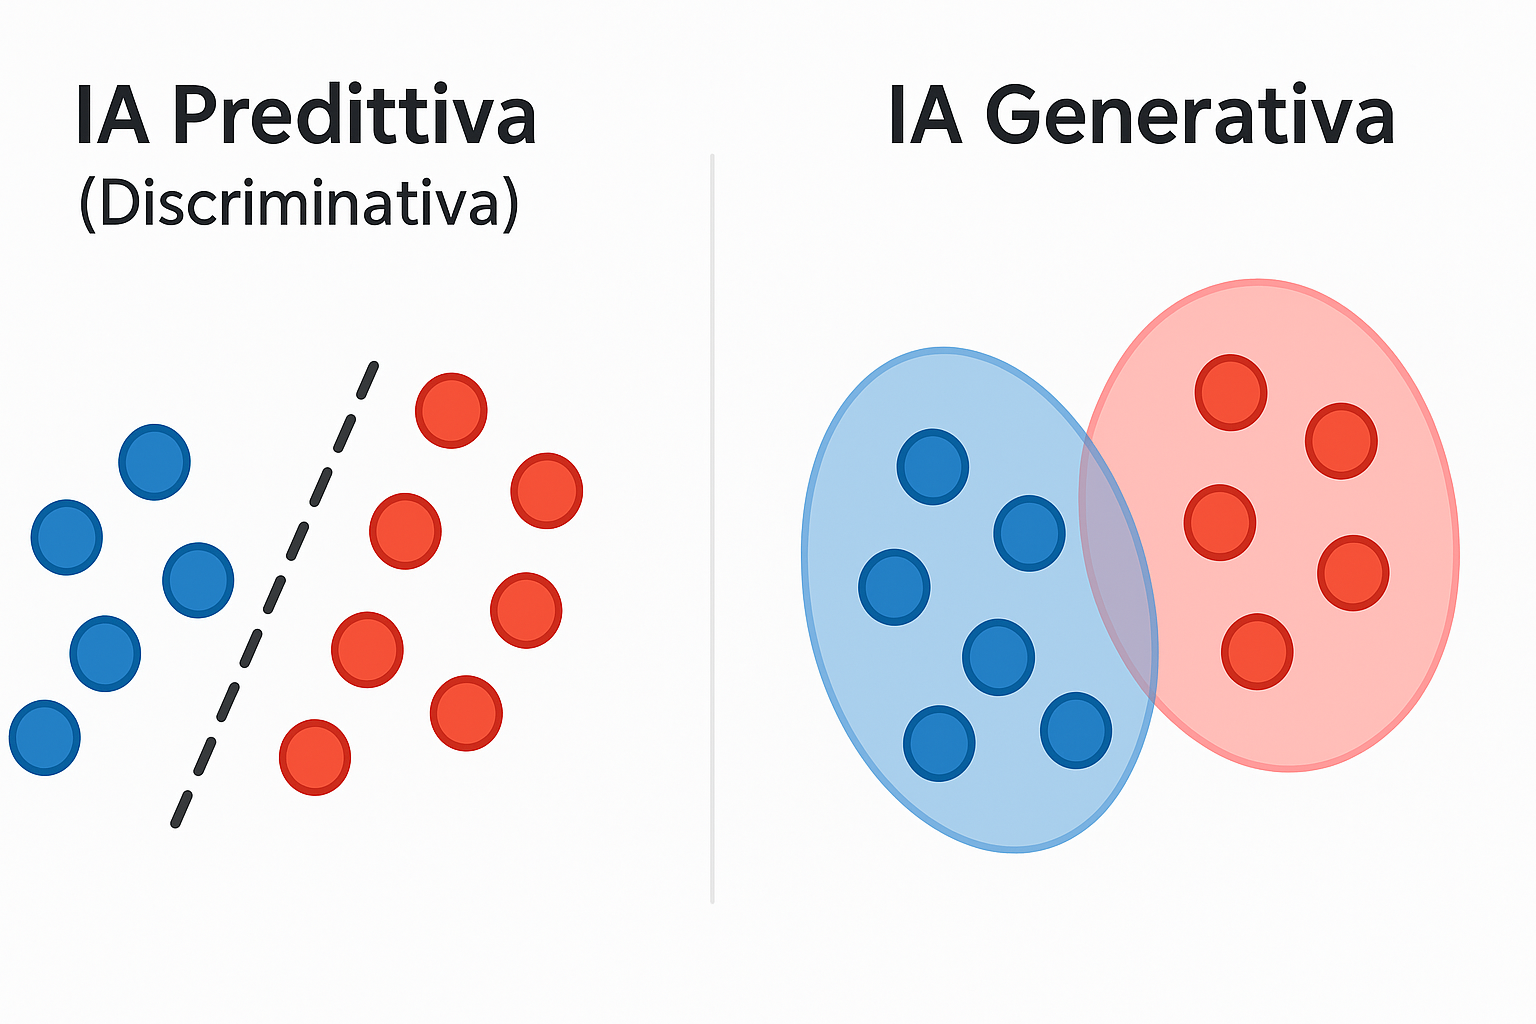
\includegraphics[width=0.85\textwidth]{Pic/disVSgen.png}
  \end{center}
\end{frame}

\begin{frame}{IA Predittiva – Modelli Classici}
  \begin{alertblock}{Obiettivo}
    Prevedere valori o classificazioni a partire da dati esistenti: “Cosa succederà?”
  \end{alertblock}
  \begin{alertblock}{Tecniche più diffuse}
    \textbf{Regressione lineare}, \textbf{Decision Tree}, \textbf{Random Forest}, \textbf{Neural Network} offrono soluzioni consolidate per previsione e classificazione.
  \end{alertblock}
\end{frame}


\begin{frame}{Possibili modelli \cite{scikit}}
  \begin{center}
    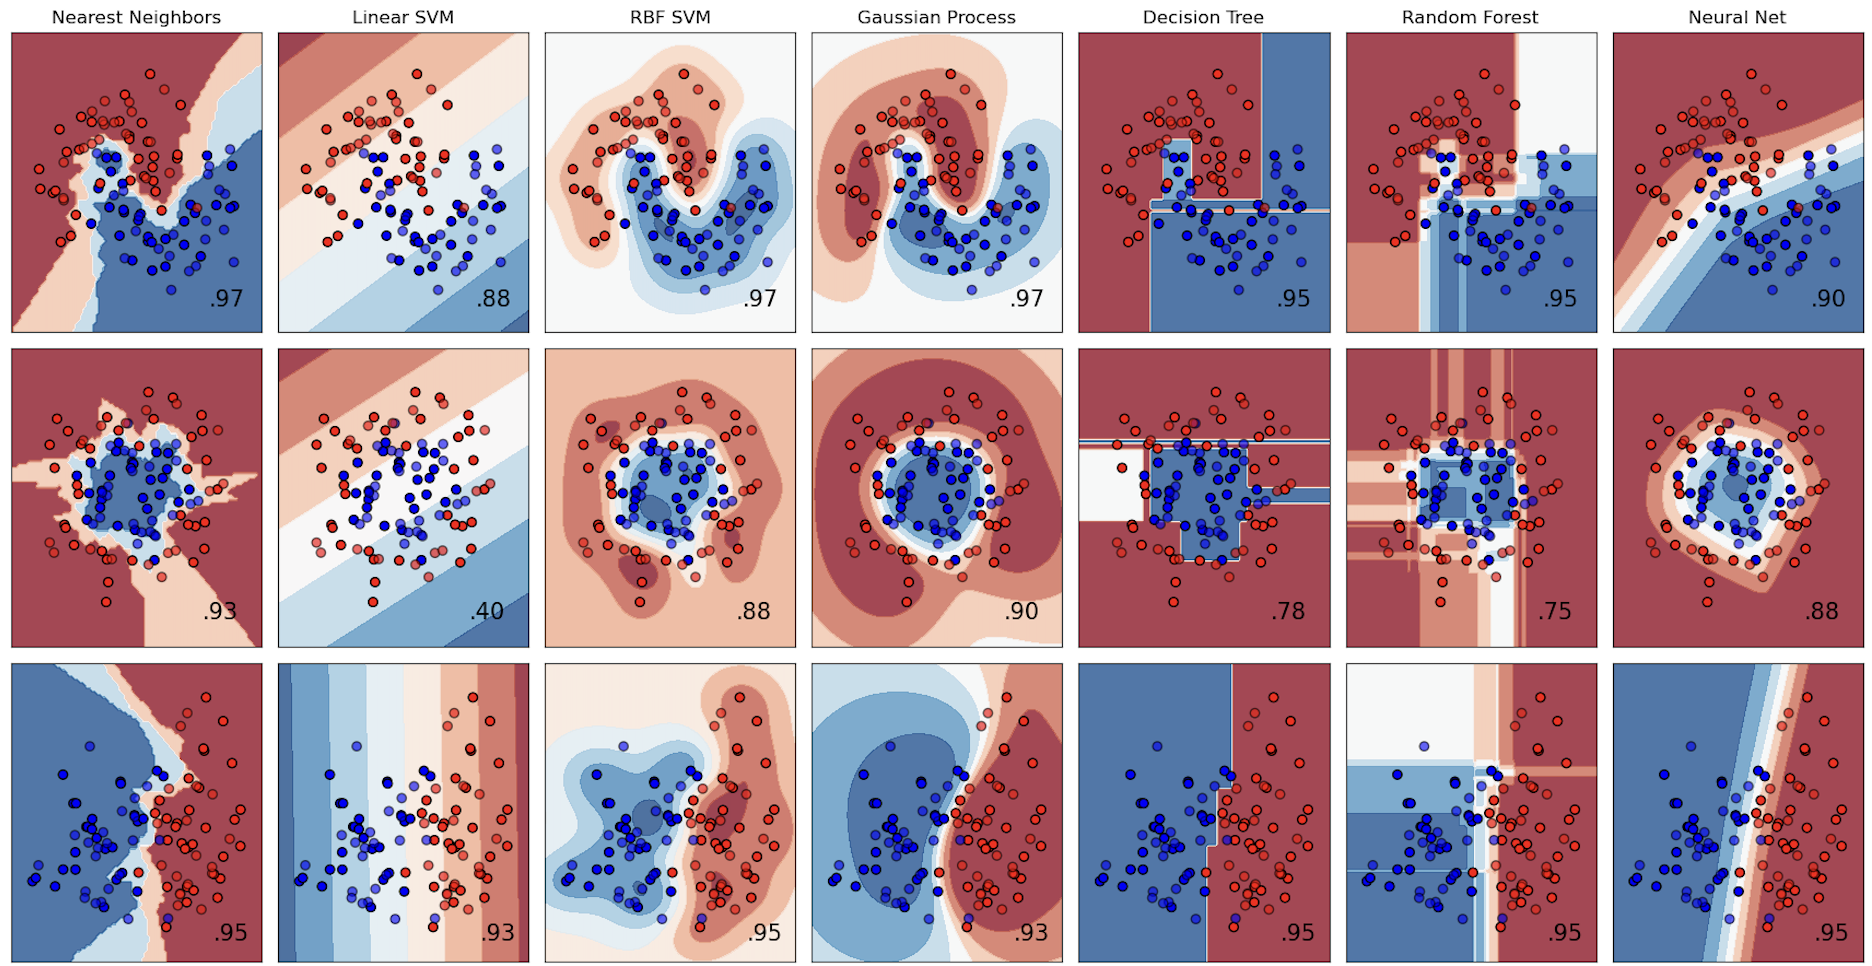
\includegraphics[width=0.85\textwidth]{Pic/dec.png}
  \end{center}
\end{frame}

\begin{frame}{Dal “Cosa Succederà?” al “Cosa Posso Creare?”}
  \begin{alertblock}{Salto concettuale}
    \textbf{Predittivo} = riempire spazi vuoti con la risposta più probabile.  
    \textbf{Generativo} = inventare da zero contenuti plausibili mai esistiti.
  \end{alertblock}
  \begin{alertblock}{Per i deepfake}
    Solo con l’IA generativa si possono creare volti, voci e scene altamente realistiche e convincenti.
  \end{alertblock}
\end{frame}

% =========================================================
\section{IA Generativa}
% =========================================================
\begin{frame}
\Huge
\begin{center}
IA Generativa
\end{center}
\end{frame}

\begin{frame}{Cos’è l’IA Generativa?}
  \begin{alertblock}{Definizione}
    Modelli che apprendono lo “stile” di un dataset (immagini, testo, audio, video) e producono nuovi esempi simili a partire da semplici prompt.
  \end{alertblock}
  \begin{alertblock}{Caratteristiche}
    Reinventano contenuti anziché selezionarli, interagiscono via testo/schizzi/audio e trovano applicazioni dall’arte alla disinformazione.
  \end{alertblock}
\end{frame}

\begin{frame}{Famiglie di Modelli Generativi}
  \begin{alertblock}{GAN – Pittore vs Critico}
    Due reti (Generatore e Discriminatore) competono fino a generare contenuti indistinguibili dalla realtà.
  \end{alertblock}
  \begin{alertblock}{VAE – Compressore Creativo}
    Encoder comprime l’input in uno spazio latente; Decoder lo ricostruisce, permettendo variazioni controllate.
  \end{alertblock}
\end{frame}

\begin{frame}{Approcci Generativi}
  \begin{alertblock}{Diffusion – Scultura dal Rumore}
    Si parte da puro rumore e si rimuove progressivamente fino a emergere un’immagine coerente e nitida.
  \end{alertblock}
  \begin{alertblock}{Transformer Autoregressivo}
    Genera token (parole, pixel, suoni) uno alla volta, preservando contesto e coerenza su lunghe sequenze.
  \end{alertblock}
\end{frame}


\begin{frame}{IA Predittiva: modelli discriminativi (TECNICA)}
\small
  \begin{alertblock}{Cosa fanno}
    \begin{itemize}
      \item Stimano la distribuzione condizionale \(\;P(y \mid x)\)\: (classificazione o regressione).
      \item Esempio: dato il profilo utente \(x\), prevedere l’età o la categoria \(\;y\).
    \end{itemize}
  \end{alertblock}
  \begin{alertblock}{Come si addestrano}
    \begin{itemize}
      \item Minimizzano la \emph{cross‐entropy} (log‐loss):
      \[
        \mathcal{L} = -\mathbb{E}_{p_{\mathrm{data}}(x,y)}\bigl[\log P(y\mid x)\bigr].
      \]
      \item Equivalente a minimizzare la divergenza di Kullback–Leibler:
      \[
        \min D_{\mathrm{KL}}\bigl(p_{\mathrm{data}}(y\mid x)\,\|\,P(y\mid x)\bigr).
      \]
      \item Intuitivamente: avvicinano la \emph{probabilità predetta} a quella \emph{osservata}.
    \end{itemize}
  \end{alertblock}
\end{frame}

\begin{frame}{IA Generativa: modelli di probabilità (TECNICA)}
\small
  \begin{alertblock}{Cosa fanno}
    \begin{itemize}
      \item Stimano la distribuzione dei dati \(\;P(x)\)\: o congiunta \(\;P(x,y)\).
      \item Permettono di \emph{campionare} nuovi esempi \(x\sim P(x)\) (immagini, testo, audio).
    \end{itemize}
  \end{alertblock}
  \begin{alertblock}{Come si addestrano}
    \begin{itemize}
      \item Massimizzano la \emph{verosimiglianza} dei dati:
      \[
        \max \mathbb{E}_{p_{\mathrm{data}}(x)}\bigl[\log P(x)\bigr]
        \;\Longleftrightarrow\;
        \min D_{\mathrm{KL}}\bigl(p_{\mathrm{data}}(x)\,\|\,P(x)\bigr).
      \]
      \item Intuitivamente: modellano \emph{l’intera forma} dei dati, non solo le etichette.
    \end{itemize}
  \end{alertblock}
\end{frame}


\begin{frame}{Approfondimento: obiettivo GAN (TECNICA) }
  \begin{alertblock}{Min–Max adversariale}
    \[
      \min_{G}\;\max_{D}\;
      V(D,G) \;=\;
      \mathbb{E}_{x\sim p_{\mathrm{data}}}\bigl[\log D(x)\bigr]
      \;+\;
      \mathbb{E}_{z\sim p_z}\bigl[\log(1 - D(G(z)))\bigr]
    \]
  \end{alertblock}
  \begin{alertblock}{Spiegazione dei termini}
    \begin{itemize}
      \item \(\mathbb{E}_{x\sim p_{\mathrm{data}}}[\log D(x)]\): il discriminatore \(D\) cerca di assegnare alta probabilità (\(\approx1\)) ai veri esempi \(x\).  
      \item \(\mathbb{E}_{z\sim p_z}[\log(1 - D(G(z)))]\): \(D\) cerca di dare bassa probabilità (\(\approx0\)) ai campioni sintetici \(G(z)\).  
      \item Il generatore \(G\) “inganna” \(D\) minimizzando \(\log(1 - D(G(z)))\), cioè vuole che \(D(G(z))\) sia alto (crede siano reali).
    \end{itemize}
  \end{alertblock}
\end{frame}


\begin{frame}{Approfondimento: obiettivo VAE (TECNICA) }
  \begin{alertblock}{Evidence Lower Bound (ELBO)}
    \[
      \log p(x)\;\ge\;
      \mathbb{E}_{z\sim q(z\mid x)}\bigl[\log p(x\mid z)\bigr]
      \;-\;
      D_{\mathrm{KL}}\bigl(q(z\mid x)\,\|\,p(z)\bigr)
    \]
  \end{alertblock}
  \begin{alertblock}{Spiegazione dei termini}
    \begin{itemize}
      \item \(\mathbb{E}_{q(z\mid x)}[\log p(x\mid z)]\): termine di \emph{ricostruzione}, misura quanto bene il decoder riproduce \(x\) dal codice \(z\).  
      \item \(D_{\mathrm{KL}}(q(z\mid x)\,\|\,p(z))\): regolarizzatore che avvicina la distribuzione latente \(q(z\mid x)\) al prior \(p(z)\) (tipicamente \(\mathcal{N}(0,I)\)).  
      \item Massimizzare ELBO = migliorare la qualità delle ricostruzioni + mantenere il latente strutturato.
    \end{itemize}
  \end{alertblock}
\end{frame}

\begin{frame}{Come VAE genera nuovi esempi (TECNICA) }
  \begin{alertblock}{Fase di campionamento}
    \begin{itemize}
      \item Si campiona \(z \sim p(z)\) (il prior, es.\ \(\mathcal{N}(0,I)\)).  
      \item Si genera \(x' \sim p(x\mid z)\) tramite il decoder.  
      \item Ogni \(x'\) è un nuovo dato plausibile secondo la distribuzione appresa.
    \end{itemize}
  \end{alertblock}
  \begin{alertblock}{Confronto con i discriminativi}
    \(\)
    \begin{itemize}
      \item \textbf{Discriminativi}: non hanno latente, non possono campionare.  
      \item \textbf{VAE}: modellano direttamente \(P(x)\) attraverso ELBO, consentendo la creazione di nuovi campioni.
    \end{itemize}
  \end{alertblock}
\end{frame}

\begin{frame}{Implicazioni per i deepfake (TECNICA)}
  \begin{alertblock}{Perché servono modelli generativi}
    \begin{itemize}
      \item Solo minimizzando \(D_{\mathrm{KL}}\bigl(p_{\mathrm{data}}(x)\,\|\,P(x)\bigr)\) si \emph{creano} contenuti nuovi e realistici.
      \item I modelli discriminativi \(P(y\mid x)\) non campionano dati: servono solo a \emph{riconoscere} o \emph{classificare}.
      \item Deepfake = generare pixel, audio o video che imitano la distribuzione reale dei media.
    \end{itemize}
  \end{alertblock}
\end{frame}



\begin{frame}{Esempi Pratici}
  \begin{alertblock}{Applicazioni Diffuse}
    Stable Diffusion (immagini da testo), ChatGPT (testo conversazionale), VALL-E (clone vocale), Make-a-Video (brief video clip).
  \end{alertblock}
\end{frame}

% =========================================================
\section{Truffe con Deepfake}
% =========================================================
\begin{frame}
\Huge
\begin{center}
Truffe con Deepfake
\end{center}
\end{frame}


\begin{frame}{Frodi Aziendali con Voice Cloning}
  \small
  \begin{alertblock}{Caso Emirati Arabi 2021}
    \begin{itemize}
      \item Deepfake audio che replica in modo quasi perfetto la voce del CEO, creato da registrazioni pregresse.
      \item Il CFO, convinto dall’autenticità, dispone un trasferimento di 35 M USD verso un conto fraudolento.\cite{brewster2021uae}\cite{darkreading_uae_deepfake}
      \item L’attacco era supportato da:
        \begin{itemize}
          \item Email di phishing estremamente mirate;  
          \item Clone vocale con accento, inflessioni e pause naturali.
        \end{itemize}
    \end{itemize}
  \end{alertblock}
\end{frame}

\begin{frame}{Frodi Aziendali con Voice Cloning}
  \small
  \begin{alertblock}{Caso Europa 2019}
    \begin{itemize}
      \item Deepfake audio del CEO generato a partire da pochi secondi di registrazione su Slack.
      \item Il reparto tesoreria, persuaso dalla corrispondenza vocale, ha eseguito un trasferimento di 220 k EUR su un conto estero.\cite{damiani2019voice}
      \item Profilo vocale così fedele da ingannare anche gli analisti di sicurezza.
    \end{itemize}
  \end{alertblock}
\end{frame}


\begin{frame}{Truffe Telefoniche Emotive}
  \begin{alertblock}{Kidnapping Scam}
    \begin{itemize}
      \item Raccolta di pochi secondi di audio di un familiare da social media.
      \item Generazione di una chiamata deepfake in cui la voce simula un sequestro e chiede aiuto.
      \item Elevato realismo emotivo spinge le vittime a versare il riscatto immediatamente.
      \item Nel 2022 FBI e FTC hanno registrato un aumento del 300 \% di questi attacchi, consigliando di adottare codici di verifica condivisi in anticipo.\cite{fbi_2022_deepfake_kidnap}\cite{ftc_2022_deepfake_kidnap}
    \end{itemize}
  \end{alertblock}
\end{frame}

\begin{frame}{Frode Cripto con Deepfake}
  \small
  \begin{alertblock}{Falso Elon Musk 2022}
    \begin{itemize}
      \item Un video deepfake mostrava Elon Musk presentare “BitVex”, piattaforma di trading cripto con “profitti garantiti” del 30 %.  
      \item L’alta qualità del volto e della voce clonata ha convinto migliaia di utenti a investire.  
      \item Si è trattato di uno schema di pump-and-dump: il valore delle token BitVex è crollato dopo la smentita ufficiale di Musk.  
      \item Dimostra come la fiducia nei personaggi pubblici possa essere sfruttata per manipolare i mercati.\cite{forbes_bitvex2022}\cite{bbc_bitvex2022}
    \end{itemize}
  \end{alertblock}
\end{frame}

% =========================================================
\section{Manipolazione dei Social Media}
% =========================================================

\begin{frame}
\Huge
\begin{center}
Manipolazione dei Social Media
\end{center}
\end{frame}

\begin{frame}{Botnet e Bot Farm}
  \small
  \begin{alertblock}{Amplificazione automatica}
    \begin{itemize}
      \item Le botnet sociali sono reti di account automatizzati che postano e condividono contenuti in massa secondo schemi prestabiliti.
      \item Uno studio dell’USC del 2020 ha rilevato che oltre il 20 \% del traffico politico su Twitter negli USA proveniva da bot \cite{uscsocial2020}.
      \item Questi bot creano “echo chamber” virtuali ripubblicando ripetutamente gli stessi messaggi, dando l’illusione di un consenso ampio \cite{echolab2020}.
      \item Manipolano gli algoritmi delle piattaforme aumentando artificialmente i livelli di engagement e influenzando la visibilità dei contenuti.
    \end{itemize}
  \end{alertblock}
\end{frame}


\begin{frame}{Like Farm e Consenso Artificiale}

  \begin{alertblock}{Fabbriche di Like}
    \begin{itemize}
      \item Le click farm impiegano operatori umani, mentre le like farm usano bot automatizzati per generare follower, like e visualizzazioni a pagamento.
      \item Un’inchiesta del 2022 in Bangladesh ha documentato giovani pagati pochi centesimi per produrre migliaia di interazioni fasulle.\cite{channel4_bangladesh}
      \item Secondo l’“Imperva 2022 Bad Bot Report”, i bot farm sfruttano proxy e account fake per eludere i filtri anti-frode delle piattaforme.\cite{imperva_badbot2022}
    \end{itemize}
  \end{alertblock}
\end{frame}

\begin{frame}{Like Farm e Consenso Artificiale}
  \begin{alertblock}{Fabbriche di Like}
    \begin{itemize}
      \item Gli algoritmi di raccomandazione amplificano questi segnali artificiali, promuovendo post e hashtag come autenticamente popolari.
      \item Implicazione politica: profili e campagne sponsorizzate ottengono visibilità ingiustificata, distorcendo il dibattito pubblico.
    \end{itemize}
  \end{alertblock}
\end{frame}

\begin{frame}{Account Falsi e Sockpuppet}
  \small
  \begin{alertblock}{Identità Inventate}
    \begin{itemize}
      \item I “sockpuppet” sono profili gestiti manualmente da operatori che usano foto e dati rubati per impersonare persone reali.
      \item Nel 2021 il Centre for Information Resilience ha smascherato 80 sockpuppet attivi su Twitter, Facebook e Instagram in India.\cite{cir2021_sockpuppet}\cite{bbc_fake_sikh}
      \item Questi account si sono infiltrati in community chiuse e gruppi di discussione per guadagnare fiducia.
      \item Una volta consolidata la reputazione, hanno iniziato a diffondere contenuti di propaganda nazionalista.
    \end{itemize}
  \end{alertblock}
\end{frame}

\begin{frame}{Comportamento Inautentico Coordinato}
  \small
  \begin{alertblock}{Operazioni su Larga Scala}
    \begin{itemize}
      \item Il Coordinated Inauthentic Behavior (CIB) unisce bot e account umani in campagne sinergiche.
      \item Nel 2021 Meta ha rimosso 52 reti CIB operanti in oltre 30 Paesi, molte con link a governi esteri o gruppi privati.\cite{meta_report}\cite{dfrlab_briefing}
      \item Tecniche utilizzate:
        \begin{itemize}
          \item Pagine esca e siti clone di testate giornalistiche.  
          \item Raccolta e rilancio sincronizzato di narrazioni su più piattaforme.
        \end{itemize}
      \item Obiettivo: manipolare il dibattito pubblico creando l’illusione di un ampio consenso.
    \end{itemize}
  \end{alertblock}
\end{frame}


% =========================================================
\section{Interferenze Politiche}
% =========================================================

\begin{frame}
\Huge
\begin{center}
Interferenze Politiche
\end{center}
\end{frame}


\begin{frame}{Interferenze Politiche: Stati Uniti}
  \small
  \begin{alertblock}{Propaganda AI‐driven}
    \begin{itemize}
      \item Dal 2023, Russia e altri attori esterni hanno diffuso video deepfake di funzionari USA; ad esempio, un falso rappresentante del Dipartimento di Stato annunciava attacchi militari inesistenti.\cite{npr_fake_us}
      \item Siti pseudo‐giornalistici come “D.C. Weekly” sono stati creati ad arte per diffondere fake news e minare la fiducia nelle fonti ufficiali.\cite{washpost_fake}
      \item Obiettivo: erodere la credibilità delle istituzioni e preparare il terreno a forme di influenza politica anche oltreoceano.
    \end{itemize}
  \end{alertblock}
\end{frame}

\begin{frame}{Interferenze Politiche: India}
  \small
  \begin{alertblock}{Deepfake in Dialetti Locali}
    \begin{itemize}
      \item Nelle elezioni di Delhi 2020 il BJP ha diffuso video deepfake in hindi e haryanvi, lingue non fluentemente parlate dal leader.\cite{india_deepfake}
      \item Sincronizzazione digitale del labiale e voce sintetica hanno creato l’illusione di un discorso diretto alle comunità locali.
    \end{itemize}
  \end{alertblock}
  \begin{alertblock}{Sockpuppet Patriottici}
    \begin{itemize}
      \item Reti di account falsi hanno veicolato messaggi nazionalisti contro dissidenti Sikh.\cite{bbc_fake_sikh}
      \item Foto rubate e narrazioni coordinate venivano usate per segmentare il pubblico e seminare discordia.
    \end{itemize}
  \end{alertblock}
\end{frame}

\begin{frame}{Interferenze Politiche: Taiwan}
  \small
  \begin{alertblock}{Operazione “Spamouflage”}
    \begin{itemize}
      \item Campagne su YouTube, Instagram e Twitter con video deepfake contro la presidente Tsai Ing-wen.\cite{taiwan_deepfake}
      \item Meta ha rimosso migliaia di account coinvolti in comportamenti inautentici coordinati.
    \end{itemize}
  \end{alertblock}
  \begin{alertblock}{Contromisure}
    \begin{itemize}
      \item Introduzione di leggi anti-deepfake durante la campagna elettorale.  
      \item Lancio di programmi di alfabetizzazione mediatica per cittadini e giornalisti.
    \end{itemize}
  \end{alertblock}
\end{frame}

\begin{frame}{Interferenze Politiche: Crisi e Conflitti}
  \small
  \begin{alertblock}{Video Fake di Zelenskyj}
    \begin{itemize}
      \item All’inizio dell’invasione russa del 2022, un deepfake di Zelenskyj annunciava la resa dell’Ucraina.\cite{zelensky_fake}
      \item Il clip fu trasmesso brevemente da un canale TV compromesso, causando disorientamento.
      \item Il vero presidente Zelenskyj smentì ufficialmente via social, ripristinando la chiarezza.
    \end{itemize}
  \end{alertblock}
\end{frame}


% =========================================================
\section{Normativa e policy}
% =========================================================
\begin{frame}{AI Act UE – Articoli 52–53}
  \begin{alertblock}{Trasparenza e Responsabilità}
    Chi diffonde contenuti “verosimili” generati o manipolati da IA deve:
    \begin{enumerate}
      \item Etichettarli chiaramente come “sintetici / AI-generated”.
      \item Conservare e rendere disponibili i metadati C2PA.
      \item Rimuovere su richiesta delle autorità in caso di illeciti (terrorismo, pornografia non consensuale, ecc.).
    \end{enumerate}
  \end{alertblock}
  \begin{alertblock}{Sanzioni}
    Fino a 35 M € o 7 \% del fatturato globale annuo, a tutela dell’integrità dell’informazione.
  \end{alertblock}
\end{frame}

\begin{frame}{Normativa Extra-UE}
  \small
  \begin{alertblock}{Panoramica Internazionale}
    \begin{itemize}
      \item \textbf{USA (FCC 2024):} vietate robocall con voce AI senza consenso scritto; multe fino a \$43 000 per chiamata.\cite{fcc_voice_2024}
      \item \textbf{UK (Online Safety Act 2023):} reato specifico per deepfake pornografici; pene fino a 2 anni di detenzione.
      \item \textbf{Italia (DDL 1146/24-25):} obbligo di etichettatura dei contenuti sintetici; multa pari al 2 \% del fatturato e obbligo di oscuramento del sito in caso di inadempienza.\cite{senato_ddl1146}
    \end{itemize}
  \end{alertblock}
\end{frame}


% =========================================================
\section{Conclusioni}
% =========================================================
\begin{frame}{Take-aways}
  \begin{alertblock}{Sintesi dei Punti Chiave}
    \begin{enumerate}
      \item \textbf{Commodity IA:} i deepfake sono oggi strumenti accessibili a molti, non solo a pochi laboratori di ricerca.
      \item \textbf{Difesa multilivello:} combinare watermark hardware, standard C2PA, educazione digitale e tecniche forensi.
      \item \textbf{Rischio real-time:} live generation di audio/video in video-chiamata (Teams, Zoom) sarà il prossimo fronte d’attacco.

    \end{enumerate}
  \end{alertblock}
\end{frame}

% =========================================================
\begin{frame}[allowframebreaks]{Riferimenti}
\printbibliography[heading=none]
\end{frame}

\end{document}


